\documentclass{article}\usepackage[]{graphicx}\usepackage[]{color}
%% maxwidth is the original width if it is less than linewidth
%% otherwise use linewidth (to make sure the graphics do not exceed the margin)
\makeatletter
\def\maxwidth{ %
  \ifdim\Gin@nat@width>\linewidth
    \linewidth
  \else
    \Gin@nat@width
  \fi
}
\makeatother

\definecolor{fgcolor}{rgb}{0.345, 0.345, 0.345}
\newcommand{\hlnum}[1]{\textcolor[rgb]{0.686,0.059,0.569}{#1}}%
\newcommand{\hlstr}[1]{\textcolor[rgb]{0.192,0.494,0.8}{#1}}%
\newcommand{\hlcom}[1]{\textcolor[rgb]{0.678,0.584,0.686}{\textit{#1}}}%
\newcommand{\hlopt}[1]{\textcolor[rgb]{0,0,0}{#1}}%
\newcommand{\hlstd}[1]{\textcolor[rgb]{0.345,0.345,0.345}{#1}}%
\newcommand{\hlkwa}[1]{\textcolor[rgb]{0.161,0.373,0.58}{\textbf{#1}}}%
\newcommand{\hlkwb}[1]{\textcolor[rgb]{0.69,0.353,0.396}{#1}}%
\newcommand{\hlkwc}[1]{\textcolor[rgb]{0.333,0.667,0.333}{#1}}%
\newcommand{\hlkwd}[1]{\textcolor[rgb]{0.737,0.353,0.396}{\textbf{#1}}}%

\usepackage{framed}
\makeatletter
\newenvironment{kframe}{%
 \def\at@end@of@kframe{}%
 \ifinner\ifhmode%
  \def\at@end@of@kframe{\end{minipage}}%
  \begin{minipage}{\columnwidth}%
 \fi\fi%
 \def\FrameCommand##1{\hskip\@totalleftmargin \hskip-\fboxsep
 \colorbox{shadecolor}{##1}\hskip-\fboxsep
     % There is no \\@totalrightmargin, so:
     \hskip-\linewidth \hskip-\@totalleftmargin \hskip\columnwidth}%
 \MakeFramed {\advance\hsize-\width
   \@totalleftmargin\z@ \linewidth\hsize
   \@setminipage}}%
 {\par\unskip\endMakeFramed%
 \at@end@of@kframe}
\makeatother

\definecolor{shadecolor}{rgb}{.97, .97, .97}
\definecolor{messagecolor}{rgb}{0, 0, 0}
\definecolor{warningcolor}{rgb}{1, 0, 1}
\definecolor{errorcolor}{rgb}{1, 0, 0}
\newenvironment{knitrout}{}{} % an empty environment to be redefined in TeX

\usepackage{alltt}
\usepackage{amssymb}
\usepackage{geometry}
\geometry{tmargin=1in,bmargin=1in,lmargin=1in,rmargin=1in}
\IfFileExists{upquote.sty}{\usepackage{upquote}}{}
\begin{document}
%\SweaveOpts{concordance=TRUE}


\title{Stat 243: Final Group Project}
\author{Sicun Huang, Cheng Ju, Fengshi Niu, Yun Zhou\\ 
        \small(in alphabetical order)}
\date{December 17, 2015}
\maketitle


% Describe the approach you took in terms of functions/modularity/object-oriented programming, and the testing that you carried out. Include a paragraph describing the specific contributions of each team member and which person/people were responsible for each component of the work. Please submit a paper copy of the document to me - either directly to me, under my door, or in my mailbox. On your paper solution, please indicate the Github user name of the group member in whose Github repository the final version of the project resides.

Please find the final version of the project in Cheng Ju's (https://github.com/jucheng1992/stat243final) Github repository .

\section{Overview}

The goal of this project is to implement an adaptive-rejection sampler for a log-concave function $f(x)$ with domain $D$ using the tangent approach. The adaptive-rejection sampling method is especially effective when function $g(x)=cf(x)$ is costly to evaluate. To reduce the number of direct computions of $g(x)$, we introduce an envelope function (i.e. the upper hull) and a squeeze function (i.e. the lower hull) and use them to construct tests to determine whether or not to accept a sample point $x$. After each test, we update the upper and lower hulls to further lower the probability of needing to evaluate $g(x)$ in the later tests. Repeat the above steps until we get a sample of $n$ points.

%------------------------------------Description of Function Modules
\section{Functions}

\subsection{Primary function $ars$ to implement the simulation}

Given a log-concave function $g(x)$ with $g(x)=cf(x)$ for some possibly unknown $c$, function $ars$ returns a sample of size $n$. 
\\[12pt]
We start by computing $h(x)$, the $log$ of $g(x)$. Then, use function $findInitAbsc$ to find the abscissae matrix comprised of the initial values of the abscissae $x_1,...x_k$ (in ascending order), together with their corresponding $h(x)$'s and $h'(x)$'s. 
\\[12pt]
From these values, we derive the unique upper and lower hull functions for $h(x)$ with functions $upperHull$ and $lowerHull$. To vectorize the following procedures, we introduce a variable $stepsize$ to denote the number of samples generated in each iteration; it increses with each iteration to accommodate for the rise in acceptance rate as test proceeds. With the $sampleUpper$ function, we generate $stepsize$ many samples from the upper hull function; compute the values of upper and lower hulls at these sample points on the original (i.e. not log) scale (denoted by $g_u$ and $g_l$). We check for log-concavity of $g(x)$ by making sure that $g_u>g_l$. Then, generate $stepsize$ many $U(0,1)$ random variables $w$'s and perform the following tests for each point:
\begin{itemize}
\item (1) If $w \leqslant \frac{g_l}{g_u}$, then accept $x$. If all $x$'s are accepted, add them to the final samples of interest; otherwise, proceed to test (2).
\item (2) Discard the $x$'s that come after the first rejected $x$. Evaluate $h(x)$ and $h'(x)$ for the first rejected $x$. If $w \leqslant \frac{exp(h(x))}{g_u}$, then accept. Add it back into the vector of accepted $x$'s and append the vector to the final samples.
\item (3) If all abscissae have zero derivatives, then the given distribution is very likely to be uniform. Thus, we will sample directly from the uniform distribution.
\end{itemize}
Use function $updateAbscissae$ to update the abscissae matrix and repeat the above steps until final sample reaches the predetermined size $n$.

\subsection{Function $findInitAbsc$ to construct the initial abscissae matrix}

Given a log-concave function $g(x)=cf(x)$, the maximum size of the abscissae $k$, and the left and right bounds of the interval on which function $g$ is defined, function $findInitAbsc$ returns a matrix comprised of the abscissae $x_1,...,x_k$ (in ascending order) and their corresponding $h(x)$'s and $h'(x)$'s, where $h(x)=log(g(x))$. 
\\[12pt]
First, we use the helper function $findMode$ to find the mode of function $h$. Notice that since the $optim$ function returns the minimum by default, we need to plug in -$h(x)$. If function $h$ is defined on $-\infty$ to $\infty$, we choose 0.5 (near center of the domain) to be the starting value (see explainations below), then use the $optim$ function with the general BFGS method to find the mode. If only one of the bounds is finite, we start near the finite bound; if both bounds are finite, we start at the middle point of the specified interval. Then we use the $optim$ function with the L-BFGS-B method to solve for the mode. To avoid complications when $g$ is distributed chi-squared, we set the upper and lower bounds to be right bound - 1e-15 and left bound + 1e-10 respectively. Notice that the global supremum can be outside of or on the boundaries of the given interval; in that case, we return the result with a warning. 
\\[12pt]
Then, we proceed to construct the abscissae. If function is defined on $-\infty$ to $\infty$, then the mode is guaranteed to be within the given interval. So we sample from both sides of the mode to obtain the desired abscissae with $h'(x_1)>0$ and $h'(x_k)<0$. If only one of the bounds is finite, we sample from the finite bound side up/down to include the mode (if mode is in the provided interval) or until we have $k$ points (if mode is not in the provided interval). If both bounds are finite, we sample with equal distance from the left bound to the right bound regardless of whether the mode is in the interval or not. With these $k$ abscissae, we compute the $h(x)$'s and $h'(x)$'s, leaving out the $x$'s with infinite $h(x)$ or $h'(x)$ values. Return the results as a matrix.
\\[12pt]
Caveats:
\begin{itemize}
\item When $g$ is distributed chi-squared with a small degree of freedom, to avoid error with the $optim$ function, we need to make sure that the starting value we plug in is not zero; if an interval is given, we use the left bound plus a small value and the right bound minus a small value as the lower and upper bounds instead of the provided values.
\item When the global supremum of $h$ is outside of or on the boundaries of the interval provided, the abscissae computed from the above method may not satisfy $h'(x_1)>0$ and $h'(x_k)<0$. Although it will still work in the later calculations.
\item When sampling from the given interval, stay away from the very edge to avoid the case where function is not defined on the boundaries.
\item It is possible for $h(x)$ and $h'(x)$ to be infinite; exclude those results to ensure that the abscissae matrix is suitable for later computations.
\item The abscissae vector needs to have at least two elements to be useful in the later calculations. If the resulted abscissae vector contains less than two points after deleting the ones with infinite $h(x)$'s or $h'(x)$'s, user may need to choose a larger $k$ value and try again.
\end{itemize}

\subsection{Function $computeZ$ to find intersections of the tangent lines}

Given the abscissae matrix, function $computeZ$ returns the intersections of the tangent lines (i.e. the kinks in the upper hull). The formula used in this function can be found in the paper by Gilks et al.
\\[12pt]
Caveats:
\begin{itemize}

\item If all derivatives $h'(x)$'s are equal, then function $h(x)$ is not strictly concave; we return a warning message as this contradicts the assumption made in Gilks et al.'s paper. However, with a user defined support interval, our package can still handle this case.

\item Some functions can be locally constant (i.e. not strictly concave), which will result in infinite $z$'s (x-coordinates for intersections of the tangent lines). In this case, we remove all infinite values from the $z$ vector, since two of the same tangent line provide no extra information.
\end{itemize}

\subsection{Functions $upperHull/lowerHull$ to find the upper/lower hull}

Given a vector $x$, functions $upperHull/lowerHull$ return the corresponding values of upper/lower hull that are uniquely defined by the abscissae matrix.
\begin{itemize}
\item For upper hull: First, we determine the intersections of the tangent lines {\em $z_j, j=1,2...k-1$} where $z_j$ is the intersection between support points $x_j$ and $x_{j+1}$. We use {\em index} to represent position in the input vector $x$, e.g. $\textrm{index[5]} = 3$ means $\mathrm{x[5] \in [ z[3-1], z[3] ]}$. After knowing the interval an $x$ falls in, we can use the corresponding piecewise linear formula to calculate its upper hull value.
\item For lower hull: Similar to upper hull, we denote position in the input vector by {\em index}, e.g. $\textrm{index[5]} = 3$ means $\mathrm{x[5] \in [ \mathbf{x}[3], \mathbf{x}[3+1] ]}$ with $\mathbf{x}$ being the vector of support points and $x$ being the input vector. After knowing the interval an $x$ falls in, we can use the corresponding piecewise linear formula to calculate its lower hull value.
\item Vectorization: To make calculations more efficient, we construct vectors $tempX1$ and $tempX2$ from the original abscissae matrix, where $tempX1$ is all support points except the first one and $tempX2$ is all support points except the last one. Then substitute them into the formula.
\end{itemize}

\noindent Problems encountered:
\begin{itemize}
\item In the $upperHull$ function, when the log density $h(x)$ is uniform or piecewise constant, we have infinite intersection $z$ values since we are dividing by 0. To see this, when the derivatives are the same at two adjacent support points, the tangent lines at the two points overlap, which result in no specific (or infinitly many) intersections. To solve this problem, we set the intersection between support points $x[i]$ and $x[i+1]$ to be $z[i] = (x[i]+x[i+1])/2$. Note that fraction $\frac{1}{2}$ is chosen arbitrarily because the intersection lies anywhere between $x[i]$ and $x[i+1]$. (See test for log piecewise constant distribution in {\em Appendix 1})
\item In the $lowerHull$ function, when a value of the input vector falls outside of the support interval, the corresponding lower hull value is negative infinity; this will cause an index overflow. To avoid this issue, we set the input values that are outside of the given interval (positions denoted by {\em mark}) to be in the interval $[ \mathbf{x}[1], \mathbf{x}[2] ]$, where $\mathbf{x}$ is a vector of the support points. This will enable us to compute all the lower hull values. We then change the lower hull values in the $mark^{th}$ position back to $- \infty $.
\item In the test function $testUpLowLogDensity$, we need to make sure that $h(x)$, upper hull, and lower hull have the same value at support points since tangent line and secant line coincide with function curve at those points. Choose 1000 random points in the support interval, and test whether or not the corresponding upper/lower hull values satisfy $upperHull \geq function h \geq lowerHull$. If not, function $h$ may not be log concave. The test cases we chose to include are Normal, Chisquare, Uniform, Piecewise constant, Exponential, and Beta distributions. (See {\em Appendix 1} for a few examples)
\item In the case where the distribution is truncated, we use the $abscissaeSummary$ function to find the adjusted range of x. Note that due to the precision problem in R, we need to be careful when comparing values of the three functions. We set the comparision precision level to be 1e10-5, which can be later adjusted in the test function.
\end{itemize}

\subsection{Function $sampleUpper$ to sample from the upper hull}

To sample from the envelope function $s(x)$ (i.e. the upper hull), we pick a random sample from the uniform distribution and transform it with the standard inverse CDF method (explained below).
\\[12pt]
We begin by generating the normalized density $exp(s(x))$, a piece-wise exponential function, from $s(x)$. In Gilks et al.'s paper, the left and right end points of the initial abscissae have positive and negative derivatives respectively. If the initial abscissae satisfy such a condition, we can solve for the inverse CDF analytically. However, we also want to deal with cases where the derivatives $h'(x)$'s are all positive or all negative over the support interval (e.g. $exp(1)$ or truncated normal). In these cases, $exp(s(x))$ diverges on the left or the right end. A workaround for this issue is to ask the user to provide the domain of $h(x)$ and set the support of $exp(s(x))$ to be the given interval. The calculations are a little bit different for the left and right end cases; we will not discuss the difference in detail here. In the end, we get the analytic expression of the inverse CDF.
\\[12pt]
The main idea for testing the inverse CDF is: for any distribution, as the range and number of elements in the abscissae increase, the envelope function grows closer to the true $h(x)$. As a result, the estimated inverse CDF gets closer to the true inverse CDF; in the limit, it converges to the true inverse CDF. Therefore, we graph the inverse CDF's derived from the envelope function and from the true distribution. If they seem to converge on the plot, then the inverse CDF passes the test. We conducted this test for exponential, chi-square (with df = 5), truncated normal, and several other distributions. The graph for truncated chi-square distribution with df = 5 is shown in $Appendix 2$.
\\[12pt]
To test the accuracy of results produced by the random sampling function, we plot the empirical CDF of a random sample with size n (generated from the envelope function) and the true CDF (constructed with a different set of initial values). If they converge on the graph as range and number of elements in the abscissae increase, the function for random sampling passes the test. We performed the test on Cauchy, chi-square, truncated normal, and some other distributions. The graph for truncated chi-square distribution with df = 5 is shown in $Appendix 3$. The figure shows that our sampling function works as expected.

\subsection{Function $updateAbscissae$ to update the abscissae matrix}

After each iteration, if we evaluated any $h$ values (e.g. in the rejection step), we want to utilize them in the future tests. For an updated set of abscissae $x$, we compute $h(x)$ and $h'(x)$, then insert them into the abscissae matrix; check that the abscissae is in increasing order with some simple tests.
\\[12pt]
Note:
\begin{itemize}
\item In the updating step, we can update lower/upper hull and inverse CDF locally. However, this does not save much time, as we are only evaluating functions that are piecewise linear or exponential in these functions. 
\item To avoid potential bugs, we only update the abscissae matrix, and use the updated matrix as input for related functions in the following iteration.
\end{itemize}

%------------------------------------
\section{Team member responsibilities}

\begin{itemize}
\item Sicun Huang (sicihuang): Write function $findInitAbs$ and its helper functions to construct the initial abscissae matrix. Write overview, ars, and findInitAbs sections in this report. Aggregate and edit report. Write and edit documentations for the package.
\item Cheng Ju (jucheng1992): Write the main adaptive rejection sampling function $ars$ and some helper functions (e.g. $computeZ$). Write test cases for the $ars$ function and other helper functions. Write report on helper and $ars$ functions. Build and test the R package.
\item Fengshi Niu (FengshiNiu): Write and test the function $upperCDFInverse$ and $sampleUpper$ to generate random variables from upper hull. 
\item Yun Zhou (YZhouEntheos): Write functions $upperHull$, $lowerHull$ and their helper functions to calculate bound values for arbitrary input vectors, $testUpLowDensity$ to inspect different cases and plot their graphs. Write test functions, documentation and report for above functions. 


\end{itemize}

\newpage
\section{Appendices}

\subsection{Appendix 1: tests}
\begin{knitrout}
\definecolor{shadecolor}{rgb}{0.969, 0.969, 0.969}\color{fgcolor}\begin{kframe}
\begin{verbatim}
## [1] "Test: log of normal distribution"
## [1] "Test passed: h function, upperhull, and lowerhull have the same value at support points"
## [1] "Test passed: upper hull always lie above the h function"
## [1] "Test passed: lower hull always lie below the h function"
## [1] "All tests passed"
## [1] "The graph is: "
\end{verbatim}
\end{kframe}
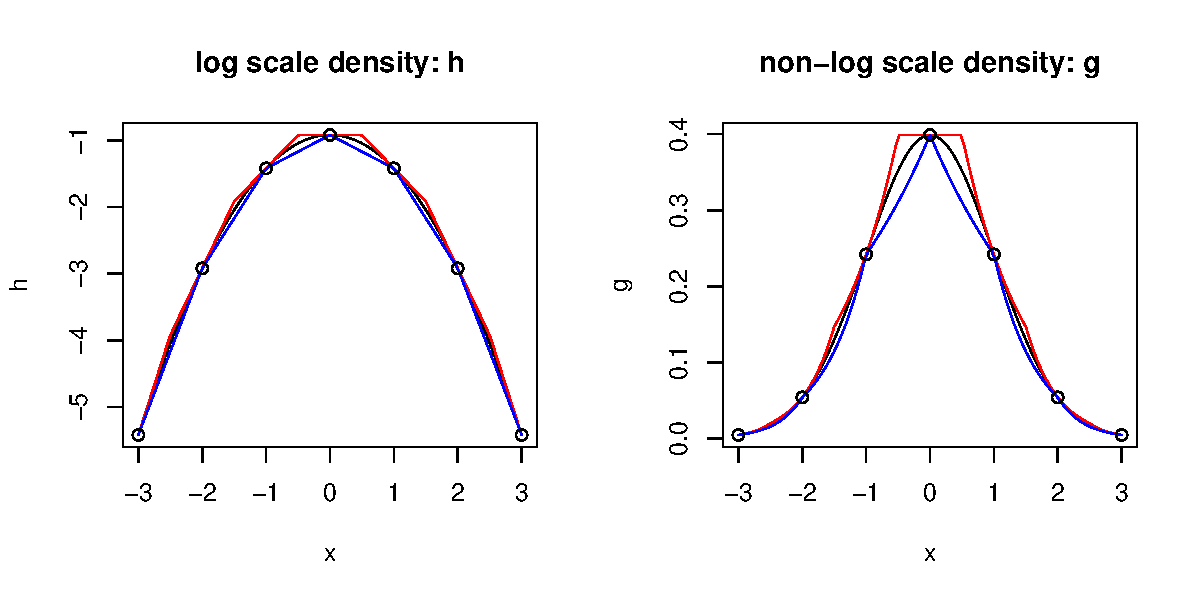
\includegraphics[width=\maxwidth]{figure/unnamed-chunk-1-1} 
\begin{kframe}\begin{verbatim}
## [1] "Test: log of beta distribution"
## [1] "Test passed: h function, upperhull, and lowerhull have the same value at support points"
## [1] "Test failed: upper hull does not always lie above the h function; h function may not be log-concave"
## [1] "Test failed: lower hull does not always lie below the h function; h function may not be log-concave"
## [1] "Some tests did not pass"
## [1] "The graph is: "
\end{verbatim}
\end{kframe}
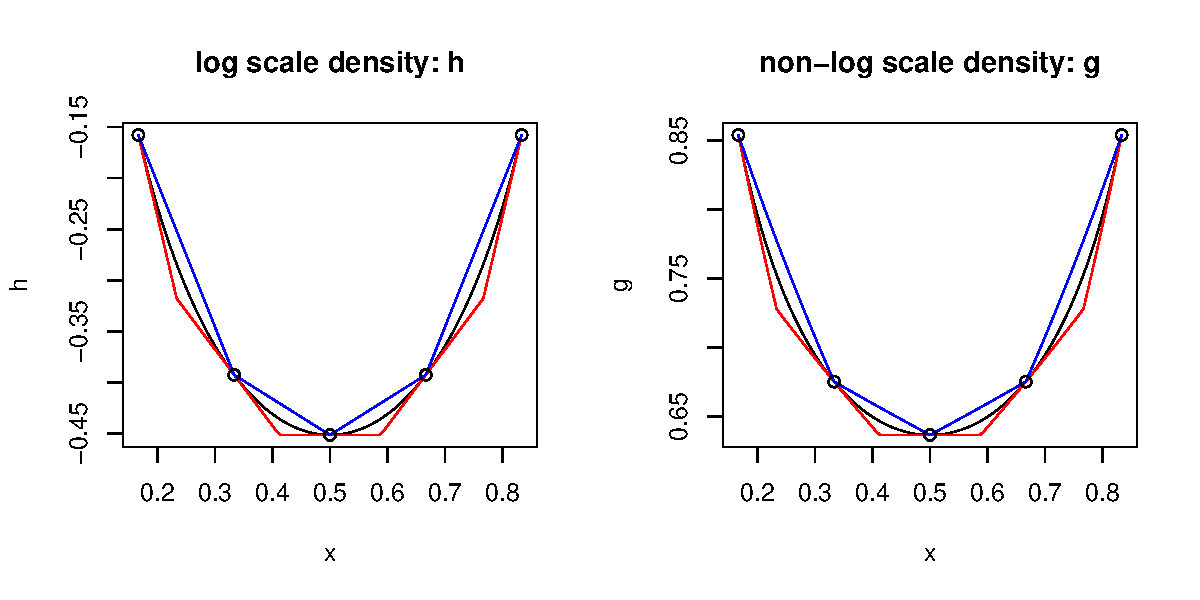
\includegraphics[width=\maxwidth]{figure/unnamed-chunk-1-2} 
\begin{kframe}\begin{verbatim}
## [1] "Test: log of uniform distribution"
## [1] "Test passed: h function, upperhull, and lowerhull have the same value at support points"
## [1] "Test passed: upper hull always lie above the h function"
## [1] "Test passed: lower hull always lie below the h function"
## [1] "All tests passed"
## [1] "The graph is: "
\end{verbatim}
\end{kframe}
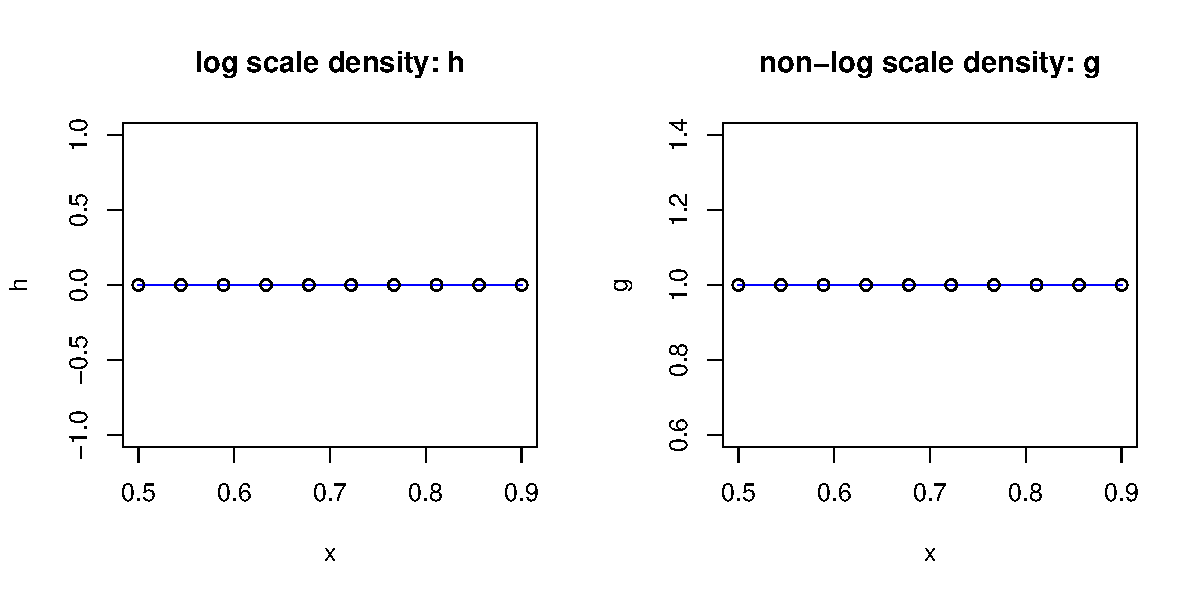
\includegraphics[width=\maxwidth]{figure/unnamed-chunk-1-3} 
\begin{kframe}\begin{verbatim}
## [1] "Test: log of piecewise-constant distribution"
## [1] "Test passed: h function, upperhull, and lowerhull have the same value at support points"
## [1] "Test passed: upper hull always lie above the h function"
## [1] "Test passed: lower hull always lie below the h function"
## [1] "All tests passed"
## [1] "The graph is: "
\end{verbatim}
\end{kframe}
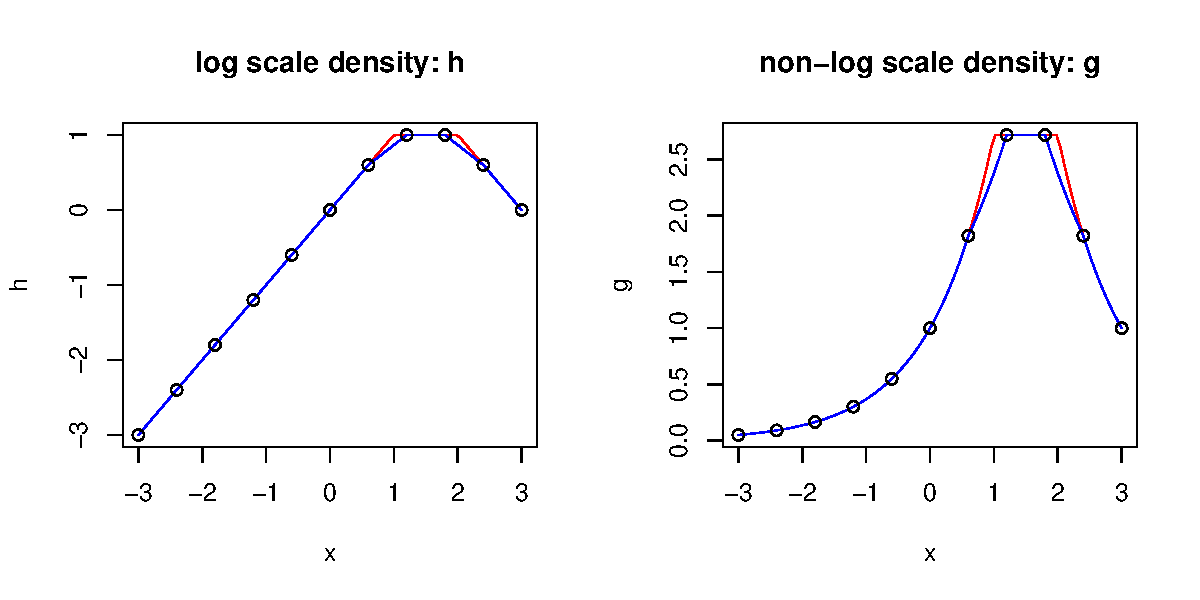
\includegraphics[width=\maxwidth]{figure/unnamed-chunk-1-4} 

\end{knitrout}

\subsection{Appendix 2}

\begin{center}
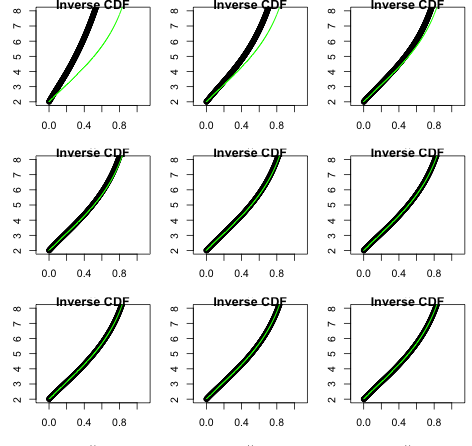
\includegraphics[width=0.7\textwidth]{figure/inverseCDFchi5}
\end{center}
\begin{center}
Figure. Inverse CDF's generated from the envelope function and the true distribution chisq 5
\end{center}

\subsection{Appendix 3}

\begin{center}
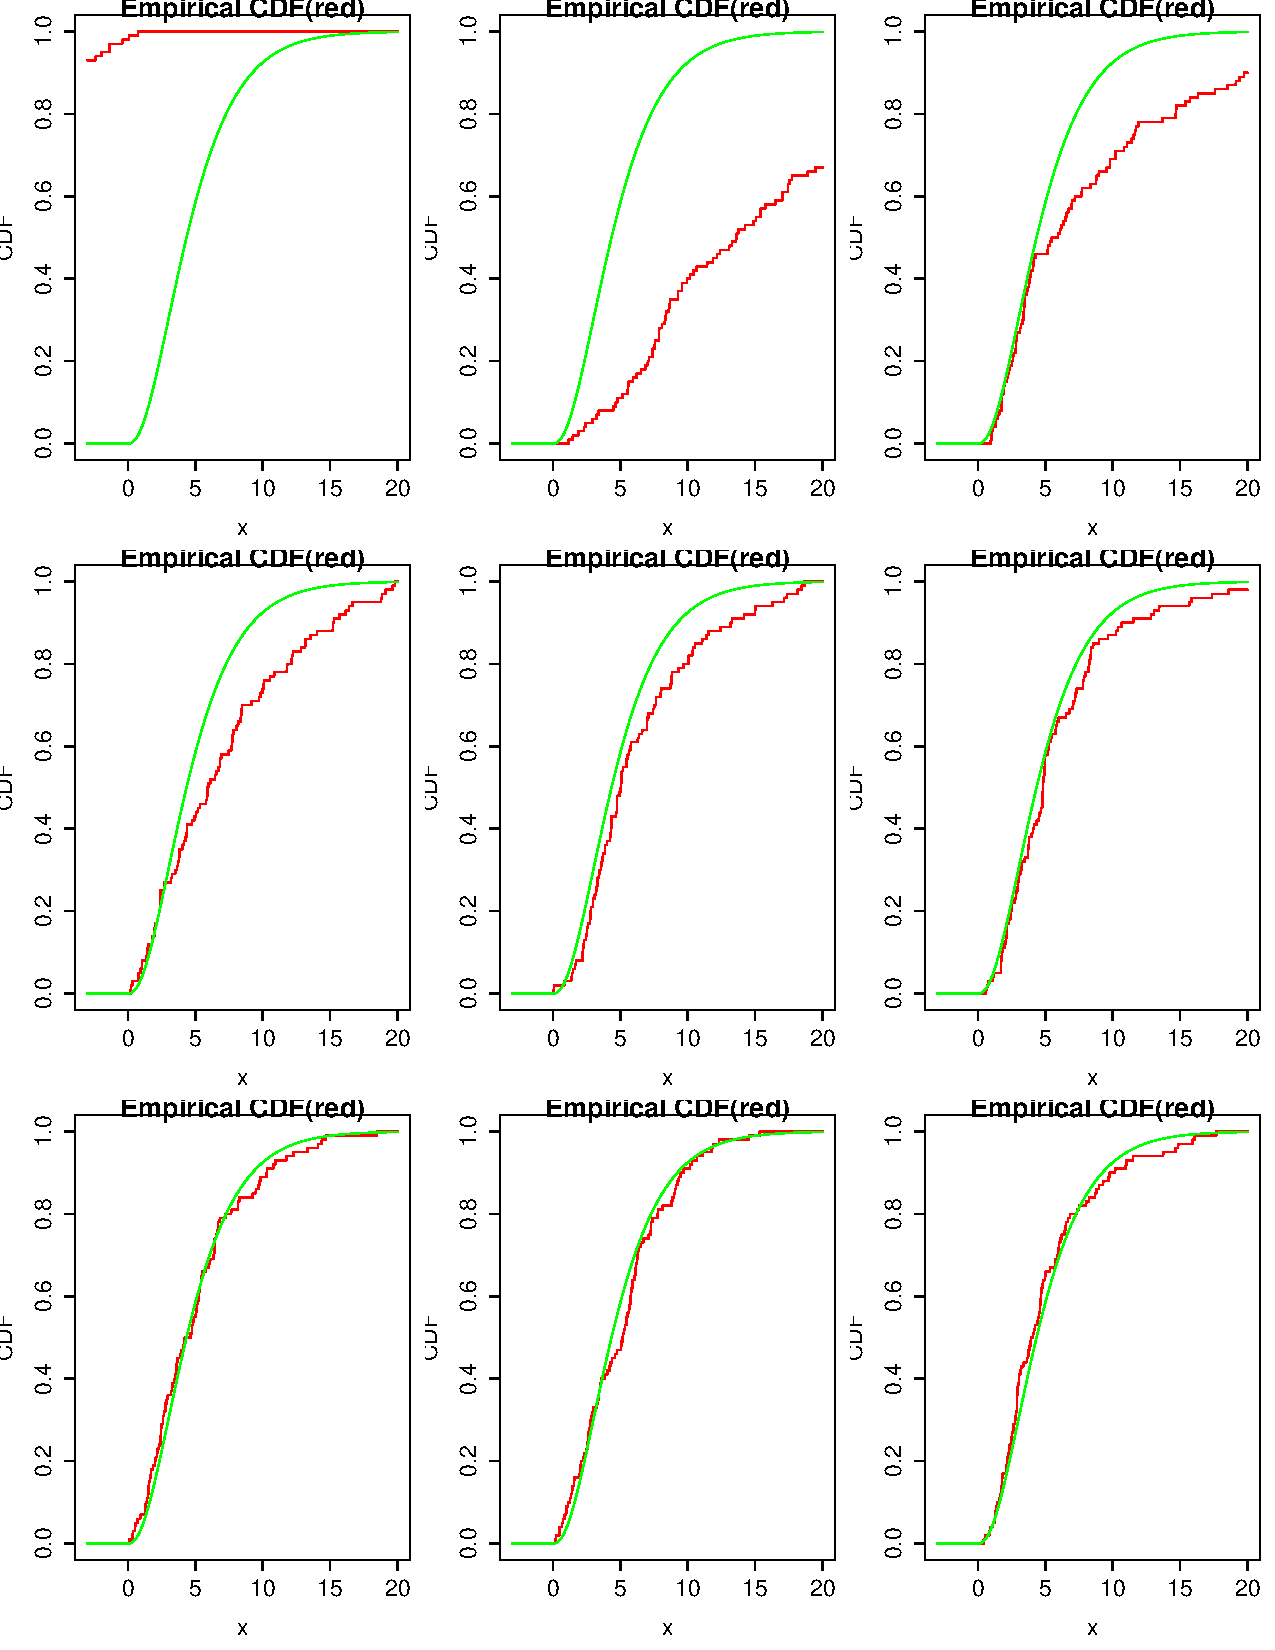
\includegraphics[width=0.7\textwidth]{figure/testUpperSample}
\end{center}
\begin{center}
Figure. The empirical CDF (generated from the envelope function) and the true CDF
\end{center}


\end{document}
